% Provenance (never printed): cycle 4 SVT, "La planete Terre, l'environnement
% et l'action humaine": resources from the Earth, their geological origin, the
% time they take to form and the rate we use them; see
% sources/book1/PROVENANCE.md. Book 1, grade 9, chapter 3.
% Vocabulary guard: owns ore deposit (with concentration factor), aggregate,
% reserve. Resource, renewable resource, ore, raw material (chemistry grade
% 5), fossil fuels (chemistry grade 8) and element abundances (chemistry
% grade 9) are recalled in prose. Groundwater and aquifers are g6's. Coal,
% oil and gas are told, not defined: "source rock", "reservoir", "seal",
% "trap" and the coal ranks belong to Book 2 g11 (fossil-fuel-geology);
% "hydrothermal" is not used (later books). Scientific notation (grade 9).
\chapter{Los recursos de la Tierra}\label{ch:g9:earth-resources}

Un teléfono inteligente cabe en un bolsillo y, sin embargo, contiene
decenas de elementos químicos: cobre para sus cables, neodimio para los
imanes de su altavoz, galio para la luz de su pantalla, indio para el fino
recubrimiento de la pantalla que conduce la electricidad, y muchos más.
Cada uno de ellos se extrajo del suelo en algún lugar de la Tierra. Una
casa contiene mucho más: una vivienda unifamiliar media necesita unas cien
toneladas de \omterm{def:g3:stones-pebbles-sand:sand}{arena}, \omterm{def:g3:stones-pebbles-sand:pebble}{grava} y piedra triturada, y su parte de las calles y
de las escuelas que la rodean, unas tres veces más. ¿En qué lugar de la
Tierra se encuentran estos materiales, y por qué allí?
% ledger: usgs:smartphone, usgs:aggregate (114 and 328 short tons: about 100 and 300 t)

\begin{recall}
En química se aprende que los materiales que tomamos de la naturaleza son
\emph{recursos}; que una \emph{mena} es una \omterm{def:g3:stones-pebbles-sand:rock}{roca} de la que se puede
extraer un metal; que un recurso \emph{renovable} es aquel que la
naturaleza renueva tan deprisa como lo usamos; que el carbón, el petróleo
y el gas natural son \emph{combustibles \omterm{def:g7:sediments-and-fossils:fossil}{fósiles}}; y que el oxígeno, el
silicio, el aluminio y el hierro son los elementos más abundantes de la
\omterm{def:g6:inside-the-earth:layers}{corteza}. El \omterm{def:g6:water-underground:groundwater}{agua subterránea} llena los \omterm{def:g6:water-underground:porosity}{poros} de un \omterm{def:g6:water-underground:aquifer}{acuífero}, y la \omterm{def:g4:clouds-rain-snow:precipitation}{lluvia}
lo recarga (\cref{ch:g6:water-underground}). Los \omterm{def:g7:sediments-and-fossils:sediment}{sedimentos} se acumulan en
capas y se convierten en \omterm{def:g6:rocks-and-minerals:rock-families}{rocas sedimentarias}
(\cref{ch:g7:sediments-and-fossils}), a lo largo de tiempos que se cuentan
en millones de años (\cref{ch:g7:geological-time}).
\end{recall}

\section{Por qué hay que concentrar un metal}

El cobre está en todas partes: una \omterm{def:g3:stones-pebbles-sand:rock}{roca} corriente contiene un poco, unos
pocos gramos por cada cien kilos. Pero para sacar un kilo de cobre de una
\omterm{def:g3:stones-pebbles-sand:rock}{roca} así habría que excavar, triturar y tratar toneladas de ella. La
minería solo compensa su coste donde la naturaleza ha reunido el metal en
una \omterm{def:g3:stones-pebbles-sand:rock}{roca} mucho más rica.
% ledger: perkins:ore-grades (copper 0.006 % of the crust)

\begin{definition}[Yacimiento mineral y factor de concentración]\label{def:g9:earth-resources:ore-deposit}
Un \emph{yacimiento mineral}\index{yacimiento mineral} es un cuerpo de
\omterm{def:g3:stones-pebbles-sand:rock}{roca} en el que procesos naturales han concentrado un metal o un \omterm{def:g6:rocks-and-minerals:mineral}{mineral} lo
suficiente para que su extracción sea rentable. El \emph{factor de
concentración}\index{factor de concentracion@factor de concentración} de
un metal es el número de veces que su contenido en la mena es mayor que su
contenido medio en la \omterm{def:g6:inside-the-earth:layers}{corteza}:
\[
\text{factor de concentración} = \frac{\text{contenido en la mena}}{\text{contenido medio en la corteza}} .
\]
\end{definition}
% ledger: perkins:ore-grades, earle:ore-grades

Los metales comunes de la \omterm{def:g6:inside-the-earth:layers}{corteza}, el aluminio y el hierro, solo necesitan
concentrarse unas cuatro veces. El cobre necesita unas 80 veces, el zinc
unas 600 veces, y los metales más escasos del gráfico, el oro, el estaño y
el cromo, miles de veces. Cuanto más escaso es un metal en la \omterm{def:g6:inside-the-earth:layers}{corteza}, más
tiene que trabajar la naturaleza para formar una mena de él, y menos son
los lugares donde lo ha hecho.
% ledger: perkins:ore-grades, earle:ore-grades

\begin{example}[El cobre]
La \omterm{def:g6:inside-the-earth:layers}{corteza} contiene de media un \qty{0.006}{\%} de cobre; una mena de
cobre puede explotarse a partir de un \qty{0.5}{\%}. El \omterm{def:g9:earth-resources:ore-deposit}{factor de
concentración} es $0.5 \div 0.006
\approx 83$, unas 80 veces, o cerca de $10^2$. Otro libro de texto toma
\qty{40}{ppm} (\qty{0.004}{\%}) para la \omterm{def:g3:stones-pebbles-sand:rock}{roca} corriente y un \qty{1}{\%}
para la mena: $1 \div
0.004 = 250$. Los dos números difieren, pero ambos dicen lo mismo: una
mena de cobre es unas cien veces más rica que la \omterm{def:g3:stones-pebbles-sand:rock}{roca} corriente.
\end{example}
% ledger: perkins:ore-grades, earle:ore-grades

\begin{omfigure}
\begin{tikzpicture}
\begin{axis}[xbar, xmode=log, width=12cm, height=5.3cm, xmin=1, xmax=2e4,
  log origin=infty, bar width=9pt, enlarge y limits=0.1,
  ytick=data, yticklabels={aluminio, hierro, cobre, zinc, oro, estaño, cromo},
  y dir=reverse, xlabel={factor de concentración (escala logarítmica)},
  xtick={1,10,100,1000,10000}, xticklabels={$1$,$10$,$10^2$,$10^3$,$10^4$},
  tick label style={font=\footnotesize}, label style={font=\small},
  nodes near coords, nodes near coords style={font=\scriptsize, anchor=west},
  point meta=explicit, xmajorgrids, grid style={black!12}]
\addplot[fill=omWarm!45, draw=omWarm!80!black] table[x=factor, y=x, meta=factor] {figdata/out/grade-9-concentration.dat};
\end{axis}
\end{tikzpicture}

{\small Cuántas veces tiene que concentrar la naturaleza siete metales para
formar una mena que merezca explotarse: la ley mínima de la mena dividida
por el contenido medio de la \omterm{def:g6:inside-the-earth:layers}{corteza}. Cada paso de la escala es diez veces
el anterior. Datos: D.~Perkins y otros, \emph{Mineralogy}, y, para el oro,
S.~Earle, \emph{Environmental Geology}.}
% ledger: perkins:ore-grades, earle:ore-grades (figdata/grade-9/concentration.py)
\label{fig:g9:earth-resources:factors}
\end{omfigure}

\begin{method}[Calcular un factor de concentración]
\begin{enumerate}
  \item Escribe el contenido del metal en la mena y en la \omterm{def:g6:inside-the-earth:layers}{corteza} media en
        la misma unidad (tanto por ciento, o gramos por tonelada).
  \item Divide el contenido en la mena entre el contenido en la \omterm{def:g6:inside-the-earth:layers}{corteza}.
  \item Redondea el resultado: lo que importa es su orden de magnitud,
        unas 10, 100 o 1000 veces, que puedes escribir como una potencia de
        diez.
\end{enumerate}
\end{method}


\section{Cómo se forman los yacimientos minerales}

La naturaleza concentra los metales de varias maneras. Abajo se muestran tres de ellas.

\begin{omfigure}
\begin{tikzpicture}[x=1cm, y=1cm, font=\footnotesize, >={Stealth[length=2mm]}]
  % country rock
  \fill[black!13] (0,0) rectangle (13,4.6);
  % surface with a valley on the right
  \fill[white] (0,4.6) -- (8.4,4.6) -- (9.6,3.7) -- (11.2,3.7) -- (12.0,4.6) -- (13,4.6) -- (13,5.6) -- (0,5.6) -- cycle;
  \draw[black!60] (0,4.6) -- (8.4,4.6) -- (9.6,3.7) -- (11.2,3.7) -- (12.0,4.6) -- (13,4.6);
  % river gravels on the valley floor
  \fill[omLithCongl] (9.5,3.75) -- (11.3,3.75) -- (11.15,3.35) -- (9.65,3.35) -- cycle;
  \foreach \x in {9.8,10.1,10.45,10.8,11.05} \fill[black!45] (\x,3.6) circle (0.05);
  \foreach \x in {9.9,10.3,10.65,10.95} \fill[yellow!80!orange] (\x,3.4) circle (0.045);
  \fill[omRiver!60] (9.9,3.75) rectangle (10.9,3.85);
  % magma body (cooling granite)
  \fill[omLithGranite] (1.0,0) .. controls (1.2,1.6) and (2.2,2.1) .. (3.4,2.1)
     .. controls (4.6,2.1) and (5.6,1.6) .. (5.8,0) -- cycle;
  \draw[black!50] (1.0,0) .. controls (1.2,1.6) and (2.2,2.1) .. (3.4,2.1)
     .. controls (4.6,2.1) and (5.6,1.6) .. (5.8,0);
  % heavy minerals settled at the bottom of the magma body
  \fill[black!60] (1.05,0) rectangle (5.75,0.25);
  % cracks and veins above the magma
  \foreach \x/\a in {2.6/12, 3.4/-6, 4.3/-15} {
    \draw[black, line width=1.6pt] (\x,2.15) -- ++(90+\a:2.0);
    \draw[yellow!80!orange, line width=0.6pt] (\x,2.15) -- ++(90+\a:2.0);
  }
  % hot water rising
  \draw[->, omWarm, thick] (2.1,1.9) .. controls (1.9,2.7) and (2.2,3.2) .. (2.45,3.7);
  \draw[->, omWarm, thick] (4.95,1.7) .. controls (5.1,2.6) and (4.8,3.3) .. (4.55,3.8);
  % labels
  \node[anchor=north, align=center] at (3.4,1.35) {un cuerpo de magma que se enfría};
  \node[anchor=west, align=left, fill=white, fill opacity=0.85, text opacity=1, inner sep=1.5pt] at (6.2,0.75)
    {\textbf{1} los minerales pesados ricos en\\ metales se depositan en el fondo};
  \draw[black!70] (6.15,0.65) -- (5.5,0.15);
  \node[anchor=west, align=left, fill=white, fill opacity=0.85, text opacity=1, inner sep=1.5pt] at (5.6,2.55)
    {\textbf{2} el agua caliente sube por las grietas,\\ se enfría y deja metales: filones};
  \draw[black!70] (5.55,2.6) -- (4.2,3.3);
  \node[anchor=south, align=center] at (10.4,4.7) {\textbf{3} los granos de oro se depositan con\\ la grava de un río: un placer};
  \draw[black!70] (10.4,4.7) -- (10.3,3.45);
  \node[anchor=south west] at (0.1,4.65) {superficie del suelo};
\end{tikzpicture}

{\small Tres maneras de concentrar un metal (un esquema, no a escala).
(1) En un cuerpo de \omterm{def:g7:volcanoes:magma}{magma}, los \omterm{def:g6:rocks-and-minerals:mineral}{minerales} pesados ricos en níquel o en
cobre se hunden y se acumulan en el fondo. (2) El \omterm{def:g6:water-underground:groundwater}{agua subterránea}
calentada por el \omterm{def:g7:volcanoes:magma}{magma}, y el agua que desprende el propio \omterm{def:g7:volcanoes:magma}{magma}, disuelven
metales, suben por las grietas y los depositan donde la \omterm{def:g3:stones-pebbles-sand:rock}{roca} está más
fría, rellenando las grietas con filones. (3) La \omterm{def:g5:water-shapes-the-land:erosion}{erosión} libera el oro de
los filones; el \omterm{def:g1:landscapes-around-us:water}{río} lo transporta, y los granos pesados se depositan entre
las \omterm{def:g3:stones-pebbles-sand:pebble}{gravas}, hasta la \omterm{def:g3:stones-pebbles-sand:rock}{roca} madre.}
% ledger: earle:magmatic, usgs:gold-lode, usgs:gold-placer
\label{fig:g9:earth-resources:deposits}
\end{omfigure}

\paragraph{En el magma.} Cuando un cuerpo de \omterm{def:g7:volcanoes:magma}{magma} se enfría, los
\omterm{def:g6:rocks-and-minerals:mineral}{minerales} que cristalizan primero no siempre son los más ligeros. En los
\omterm{def:g7:volcanoes:magma}{magmas} procedentes del \omterm{def:g6:inside-the-earth:layers}{manto}, los \omterm{def:g6:rocks-and-minerals:mineral}{minerales} pesados ricos en níquel y en
cobre se hunden hasta el fondo y se acumulan en una capa rica. La mayor
parte del níquel que se extrae en el mundo procede de yacimientos de este
tipo.
% ledger: earle:magmatic

\paragraph{En las grietas, a partir de agua caliente.} El \omterm{def:g6:water-underground:groundwater}{agua
subterránea} que circula cerca de un cuerpo de \omterm{def:g7:volcanoes:magma}{magma}, a unos pocos
kilómetros bajo la superficie, se calienta y sube por las grietas de la
\omterm{def:g3:stones-pebbles-sand:rock}{roca}. El agua caliente disuelve metales de las \omterm{def:g3:stones-pebbles-sand:rock}{rocas} que atraviesa. Cuando
llega a una \omterm{def:g3:stones-pebbles-sand:rock}{roca} más fría, más cerca de la superficie, los metales salen
del agua en forma de \omterm{def:g6:rocks-and-minerals:mineral}{minerales} y rellenan las grietas: son los
\emph{filones}\index{filon@filón}. Muchos yacimientos de oro son filones de
este tipo. Alrededor de algunos cuerpos de \omterm{def:g7:volcanoes:magma}{magma}, el agua caliente ha
atravesado toda una masa de \omterm{def:g3:stones-pebbles-sand:rock}{roca} fracturada y ha dejado en ella cobre,
disperso pero en un volumen enorme: son los mayores yacimientos de cobre
del mundo.
% ledger: usgs:gold-lode, earle:porphyry

\begin{omfigure}
\begin{minipage}[c]{0.46\linewidth}\centering
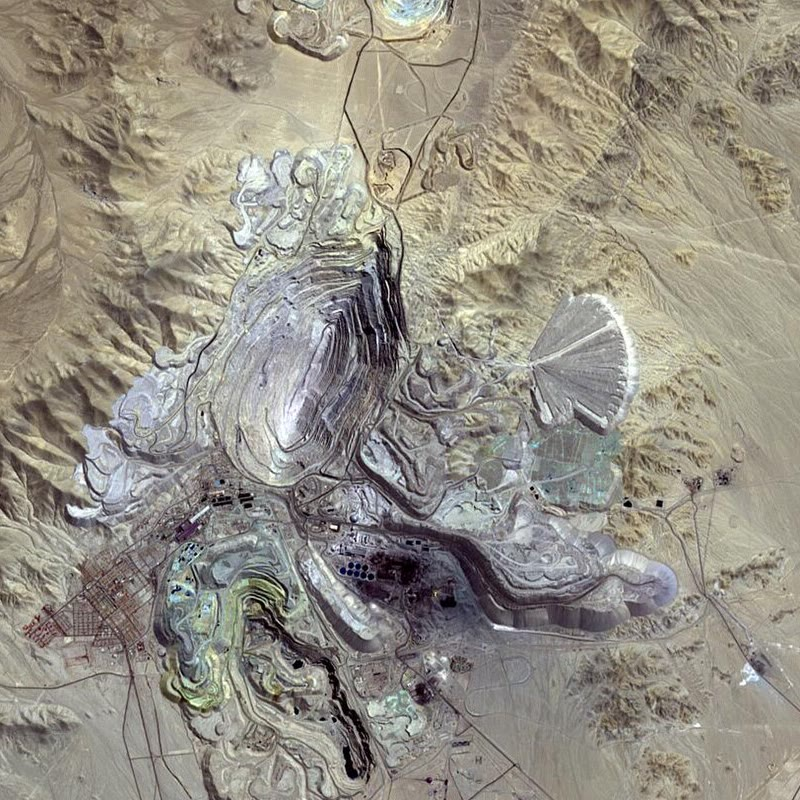
\includegraphics[width=\linewidth]{images/book1/g9-chuquicamata.jpg}
\end{minipage}\hfill
\begin{minipage}[c]{0.5\linewidth}\raggedright
{\small La mina de cobre de Chuquicamata, en el \omterm{def:g5:weather-and-climate:desert}{desierto} de Atacama, en
Chile, vista por el instrumento ASTER de un satélite de la NASA en 2007
(la imagen abarca unos \qty{12}{km}). La corta ovalada del centro,
explotada desde hace más de un siglo, mide \qty{4.3}{km} de largo,
\qty{2.7}{km} de ancho y \qty{1.1}{km} de profundidad. NASA/METI/AIST/Japan
Space Systems y U.S./Japan ASTER Science Team (dominio público, vía
Wikimedia Commons).}
\end{minipage}
% ledger: commons:chuquicamata, earle:chuquicamata
\label{fig:g9:earth-resources:chuquicamata}
\end{omfigure}

\paragraph{En las gravas de los ríos.} El oro no se oxida y apenas se
altera. Cuando la \omterm{def:g5:water-shapes-the-land:erosion}{erosión} desgasta un filón de oro, el oro se libera en
forma de polvo, escamas, granos y a veces pepitas, y los \omterm{def:g1:landscapes-around-us:water}{ríos} lo
transportan aguas abajo. El oro es muy denso: unos \qty{19}{g/cm^3} puro,
frente a unos \qty{2.5}{g/cm^3} de la \omterm{def:g3:stones-pebbles-sand:rock}{roca} corriente. En las \omterm{def:g5:water-shapes-the-land:flood}{crecidas},
cuando todo el lecho de \omterm{def:g3:stones-pebbles-sand:sand}{arena} y \omterm{def:g3:stones-pebbles-sand:pebble}{grava} se mueve, los granos pesados de oro
se abren paso hacia abajo y se acumulan sobre la \omterm{def:g3:stones-pebbles-sand:rock}{roca} madre. Los geólogos
llaman a estos yacimientos \emph{placeres}\index{placer}.
% ledger: usgs:gold-placer

\section{Carbón, petróleo y gas}

El carbón, el petróleo y el gas natural son restos de seres vivos,
enterrados antes de que pudieran pudrirse. Casi toda la materia orgánica
de una planta o de un animal muertos vuelve a transformarse en dióxido de
carbono en unas semanas o unas décadas. Solo la parte aislada del oxígeno
del aire, en el fondo de un pantano de aguas estancadas o de un \omterm{def:g2:water-on-earth:ocean}{mar}
profundo, puede quedar enterrada y conservarse durante millones de años.
% ledger: earle:coal, earle:oil-gas

\begin{omfigure}
\begin{minipage}[c]{0.46\linewidth}\centering
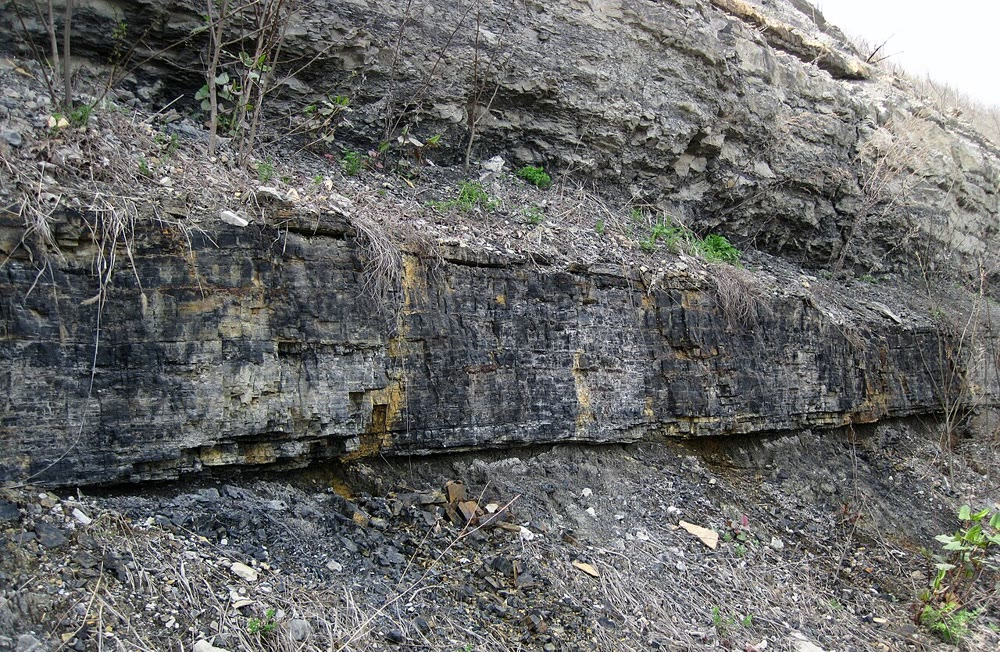
\includegraphics[width=\linewidth]{images/book1/g9-coal-seam.jpg}
\end{minipage}\hfill
\begin{minipage}[c]{0.5\linewidth}\raggedright
{\small Una capa de carbón, la franja oscura que cruza el centro, entre
\omterm{def:g6:rocks-and-minerals:rock-families}{rocas sedimentarias}, junto a una carretera de Ohio, en Estados Unidos. La
capa está horizontal, como lo estaba el pantano. Fotografía de James
St.~John (CC BY 2.0, vía Wikimedia Commons).}
\end{minipage}
% ledger: commons:meigs-coal
\label{fig:g9:earth-resources:coal-seam}
\end{omfigure}


\paragraph{El carbón.} El carbón empieza en los pantanos que bordean \omterm{def:g1:landscapes-around-us:water}{ríos}
y \omterm{def:g5:water-shapes-the-land:delta}{deltas}, en \omterm{def:g5:weather-and-climate:climate}{climas} cálidos y húmedos, donde las plantas crecen deprisa.
Los troncos y las hojas muertos caen en un agua quieta que contiene poco
oxígeno, y no se pudren. El pantano tiene que durar de siglos a milenios
para formar una capa gruesa. Un día, un \omterm{def:g1:landscapes-around-us:water}{río} cambia de curso o se
desborda, y cubre el pantano de \omterm{def:g3:stones-pebbles-sand:sand}{arena} y \omterm{def:g3:stones-pebbles-sand:sand}{barro}. A medida que se acumulan
más \omterm{def:g7:sediments-and-fossils:sediment}{sedimentos}, la capa vegetal se comprime y se calienta, y se transforma
en carbón: primero un carbón pardo y blando, con alrededor de un tercio de
carbono, a unos cientos de metros de profundidad; después un carbón negro
y duro, con hasta un 86~\% de carbono, a unos pocos kilómetros. El carbón
que se extrae hoy en Estados Unidos, por ejemplo, tiene en su mayoría de
100 a 300~millones de años.
% ledger: earle:coal, eia:coal

\begin{omfigure}
\begin{tikzpicture}[x=1cm, y=0.8cm, font=\footnotesize]
  \foreach \i/\t in {0/{(a) bosque pantanoso:\\ las plantas muertas\\ se acumulan bajo\\ el agua quieta},
                     1/{(b) enterrada bajo\\ arena y barro de río,\\ la capa se comprime},
                     2/{(c) más hondo\\ y más caliente\\ (cientos de metros):\\ carbón pardo y blando},
                     3/{(d) más hondo todavía\\ (kilómetros):\\ carbón negro y duro}} {
    \begin{scope}[xshift=\i*3.35cm]
      \draw[black!40] (0,0) rectangle (2.9,4.2);
      \node[align=center, anchor=north, font=\scriptsize] at (1.45,-0.1) {\t};
    \end{scope}
  }
  % (a) swamp: water, trees, plant layer
  \fill[omSea] (0,2.6) rectangle (2.9,3.1);
  \fill[brown!60!black!70] (0,2.0) rectangle (2.9,2.6);
  \fill[omLithShale] (0,0) rectangle (2.9,2.0);
  \foreach \x in {0.5,1.4,2.3} {
    \draw[brown!50!black, line width=1.2pt] (\x,2.6) -- (\x,3.7);
    \fill[green!45!black] (\x,3.85) circle (0.3);
  }
  % (b) buried
  \begin{scope}[xshift=3.35cm]
    \fill[lith sandstone] (0,2.6) rectangle (2.9,4.0);
    \fill[brown!55!black!80] (0,2.2) rectangle (2.9,2.6);
    \fill[omLithShale] (0,0) rectangle (2.9,2.2);
    \draw[->, thick] (1.45,4.15) -- (1.45,3.45);
  \end{scope}
  % (c) lignite
  \begin{scope}[xshift=6.7cm]
    \fill[lith sandstone] (0,1.9) rectangle (2.9,4.2);
    \fill[brown!45!black] (0,1.65) rectangle (2.9,1.9);
    \fill[omLithShale] (0,0) rectangle (2.9,1.65);
  \end{scope}
  % (d) coal
  \begin{scope}[xshift=10.05cm]
    \fill[lith sandstone] (0,1.25) rectangle (2.9,4.2);
    \fill[black!85] (0,1.1) rectangle (2.9,1.25);
    \fill[omLithShale] (0,0) rectangle (2.9,1.1);
  \end{scope}
\end{tikzpicture}

{\small De un pantano a una capa de carbón (un esquema, no a escala). A
medida que la capa de plantas se hunde más, se comprime y se calienta:
pierde agua y gases, se vuelve más delgada y su proporción de carbono
aumenta.}
% ledger: earle:coal, eia:coal
\label{fig:g9:earth-resources:coal}
\end{omfigure}


\paragraph{El petróleo y el gas.} El petróleo y la mayor parte del gas
natural proceden de las diminutas plantas y animales que viven en el \omterm{def:g2:water-on-earth:ocean}{mar},
como las diatomeas. Sus restos se hunden con el \omterm{def:g3:stones-pebbles-sand:sand}{barro} hasta el fondo del
\omterm{def:g2:water-on-earth:ocean}{mar}, y algunos quedan enterrados antes de descomponerse. Millones de años
y kilómetros de \omterm{def:g7:sediments-and-fossils:sediment}{sedimentos} después, el calor y la presión los transforman:
por debajo de unos \qty{2}{km}, entre unos 60 y \qty{120}{\degreeCelsius},
en petróleo; a temperaturas más altas todavía, en gas. El petróleo y el
gas son más ligeros que el agua. Ascienden lentamente a través de los
\omterm{def:g6:water-underground:porosity}{poros} de las \omterm{def:g3:stones-pebbles-sand:rock}{rocas} \omterm{def:g6:water-underground:permeability}{permeables}, y muchos llegan a la superficie y se
pierden. Los que encontramos fueron detenidos en su camino por una capa de
\omterm{def:g3:stones-pebbles-sand:rock}{roca} \omterm{def:g6:water-underground:permeability}{impermeable}, a menudo en lo alto de un pliegue abombado hacia arriba,
donde se acumulan: el gas arriba, el petróleo debajo y el agua más abajo.
% ledger: eia:oil, eia:gas, earle:oil-gas

\begin{omfigure}
\begin{tikzpicture}[x=1cm, y=1cm, font=\footnotesize, >={Stealth[length=2mm]}]
  \def\fold#1{(0,#1) .. controls (3,#1+1.0) and (4.0,#1+1.6) .. (6,#1+1.6) .. controls (8.0,#1+1.6) and (9,#1+1.0) .. (12,#1)}
  % layers from the bottom up
  \fill[omLithShale!60!black!40] (0,0) -- \fold{0.9} -- (12,0) -- cycle;
  \fill[lith sandstone] \fold{0.9} -- (12,2.1) -- (12,2.1) .. controls (9,3.1) and (8.0,3.7) .. (6,3.7) .. controls (4.0,3.7) and (3,3.1) .. (0,2.1) -- cycle;
  \fill[lith shale] (0,2.1) .. controls (3,3.1) and (4.0,3.7) .. (6,3.7) .. controls (8.0,3.7) and (9,3.1) .. (12,2.1) -- (12,3.6) .. controls (9,4.6) and (8.0,5.2) .. (6,5.2) .. controls (4.0,5.2) and (3,4.6) .. (0,3.6) -- cycle;
  \fill[lith sandstone] (0,3.6) .. controls (3,4.6) and (4.0,5.2) .. (6,5.2) .. controls (8.0,5.2) and (9,4.6) .. (12,3.6) -- (12,5.6) -- (0,5.6) -- cycle;
  % gas and oil under the crest of the impermeable layer
  \fill[omWxSun!60] (4.55,3.55) .. controls (5.2,3.69) and (6.8,3.69) .. (7.45,3.55) -- (7.1,3.35) -- (4.9,3.35) -- cycle;
  \fill[black!75] (4.9,3.35) -- (7.1,3.35) -- (8.05,3.05) .. controls (7.0,3.15) and (5.0,3.15) .. (3.95,3.05) -- cycle;
  % arrows: oil creeping up through the permeable layer
  \draw[->, black, thick] (1.4,2.05) -- (2.4,2.55);
  \draw[->, black, thick] (10.6,2.05) -- (9.6,2.55);
  \draw[->, black!70] (3.0,2.65) -- (3.8,2.95);
  \draw[->, black!70] (9.0,2.65) -- (8.2,2.95);
  % labels
  \node[anchor=west, fill=white, fill opacity=0.85, text opacity=1, inner sep=1.5pt] at (0.1,0.45) {barro oscuro del antiguo fondo marino: aquí se forman el petróleo y el gas};
  \node[anchor=east, fill=white, fill opacity=0.85, text opacity=1, inner sep=1.5pt] at (11.9,1.9) {arenisca permeable};
  \node[anchor=east, fill=white, fill opacity=0.85, text opacity=1, inner sep=1.5pt] at (11.9,3.25) {lutita impermeable};
  \node[anchor=south, fill=white, fill opacity=0.85, text opacity=1, inner sep=1.5pt] at (6,5.25) {rocas de superficie};
  \node[font=\scriptsize] at (6,3.48) {gas};
  \node[font=\scriptsize, text=white] at (6,3.22) {petróleo};
\end{tikzpicture}

{\small Petróleo y gas detenidos bajo una capa \omterm{def:g6:water-underground:permeability}{impermeable} en lo alto de
un pliegue abombado (un esquema, no a escala; no se muestra el agua que
llena el resto de la arenisca). Por debajo del pliegue, ascienden a través
de la arenisca \omterm{def:g6:water-underground:permeability}{permeable} (flechas) y se acumulan bajo la cresta: el gas
arriba, el petróleo debajo.}
% ledger: earle:oil-gas
\label{fig:g9:earth-resources:oil}
\end{omfigure}

\section{El agua del subsuelo}

El \omterm{def:g6:water-underground:groundwater}{agua subterránea} es también un recurso de la Tierra, el que usamos
cada día. A diferencia de un metal o del carbón, se renueva: la \omterm{def:g4:clouds-rain-snow:precipitation}{lluvia}
recarga los \omterm{def:g6:water-underground:aquifer}{acuíferos}. Pero se renueva despacio, y solo tan deprisa como
se infiltra la \omterm{def:g4:clouds-rain-snow:precipitation}{lluvia}. En un \omterm{def:g6:water-underground:aquifer}{acuífero} que se bombea más deprisa de lo que
se recarga, el \omterm{def:g6:water-underground:water-table}{nivel freático} baja y los \omterm{def:g6:water-underground:spring}{pozos} se secan
(\cref{ch:g6:water-underground}). El \omterm{def:g6:water-underground:groundwater}{agua subterránea} es un recurso
renovable solo mientras no se extraiga más deprisa de lo que se renueva.
% ledger: wss:aquifer

\section{Arena y grava}

El material sólido que más se extrae del suelo no es ni el carbón ni una
mena metálica: es la \omterm{def:g3:stones-pebbles-sand:sand}{arena} y la \omterm{def:g3:stones-pebbles-sand:pebble}{grava}.
% ledger: tos:sand

\begin{definition}[Áridos]\label{def:g9:earth-resources:aggregate}
Los \emph{áridos}\index{aridos@áridos} son la \omterm{def:g3:stones-pebbles-sand:sand}{arena}, la \omterm{def:g3:stones-pebbles-sand:pebble}{grava} y la piedra
triturada que se usan en la construcción: en el hormigón, bajo las
carreteras y las vías del tren, y para rellenar el terreno.
\end{definition}
% ledger: usgs:aggregate, tos:sand

La mayor parte de la \omterm{def:g3:stones-pebbles-sand:sand}{arena} acaba en el hormigón, una mezcla de \omterm{def:g3:stones-pebbles-sand:sand}{arena},
\omterm{def:g3:stones-pebbles-sand:pebble}{grava}, agua y cemento. En 2019, el mundo necesitaba unos 50~mil millones
de toneladas de \omterm{def:g3:stones-pebbles-sand:sand}{arena} y \omterm{def:g3:stones-pebbles-sand:pebble}{grava} al año, es decir, $5 \times 10^{10}$
toneladas, o unos \qty{18}{kg} por cada habitante de la Tierra y por día.
La \omterm{def:g3:stones-pebbles-sand:sand}{arena} y la \omterm{def:g3:stones-pebbles-sand:pebble}{grava} se extraen de graveras en tierra firme, de los lechos
de los \omterm{def:g1:landscapes-around-us:water}{ríos} y, cada vez más, del fondo del \omterm{def:g2:water-on-earth:ocean}{mar}. Cuando se sacan de un \omterm{def:g1:landscapes-around-us:water}{río},
llega menos \omterm{def:g3:stones-pebbles-sand:sand}{arena} a la \omterm{def:g1:landscapes-around-us:water}{costa}, y las playas situadas aguas abajo se
desgastan.
% ledger: tos:sand

\begin{omfigure}
\begin{minipage}[c]{0.46\linewidth}\centering
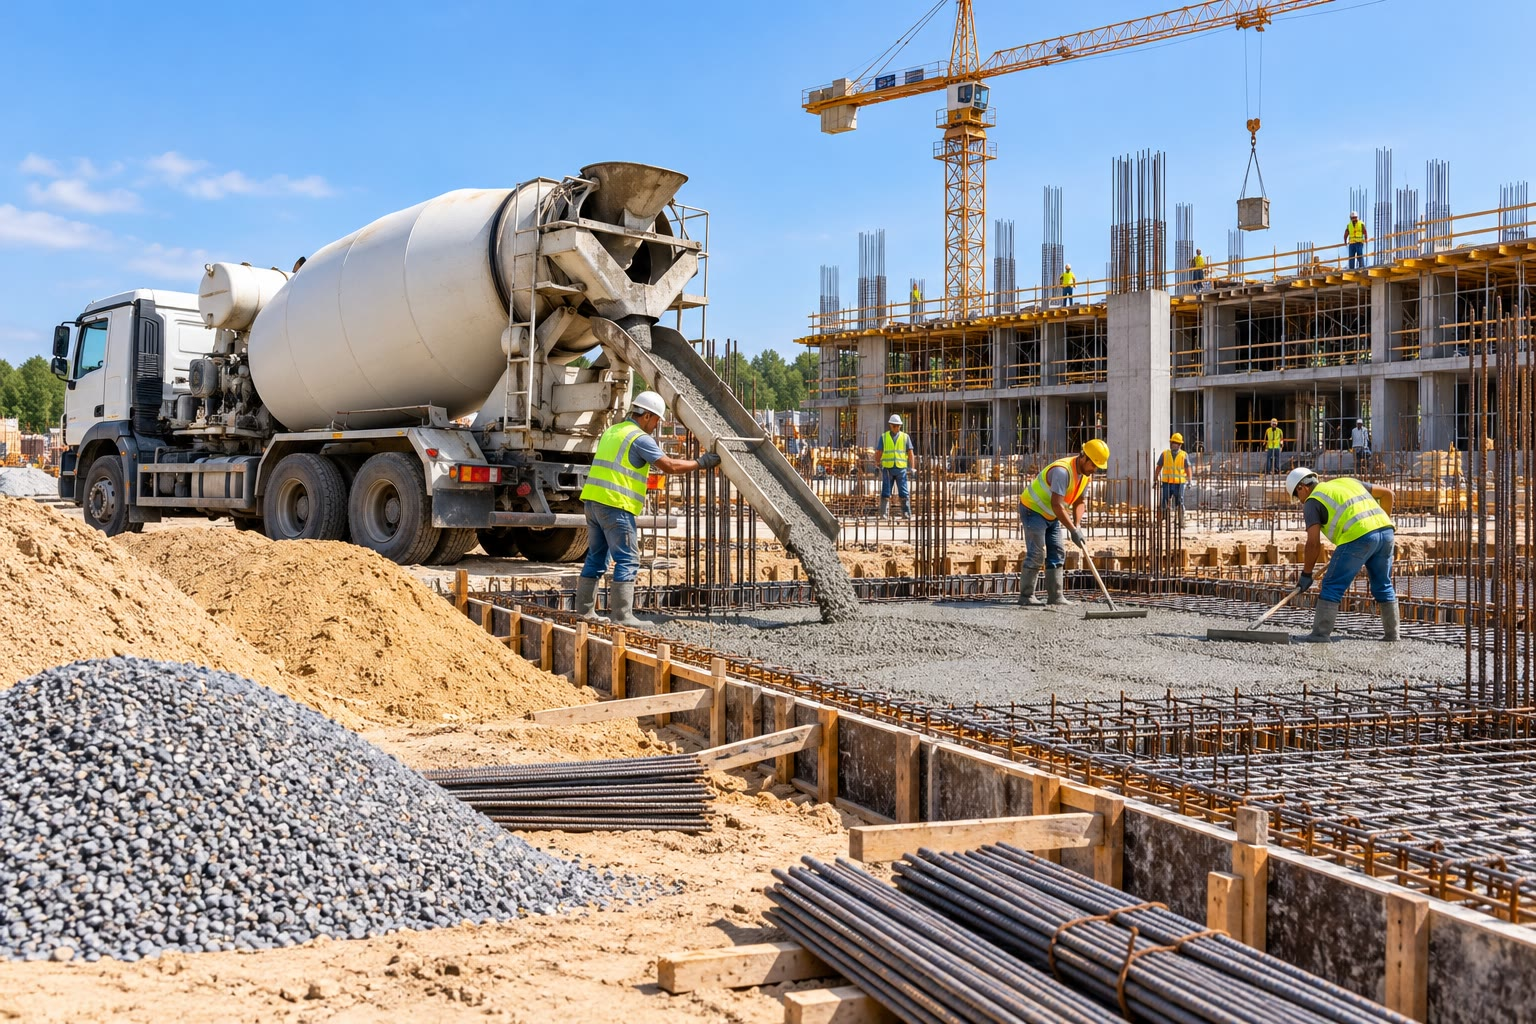
\includegraphics[width=\linewidth]{images/book1/ai/g9-building-site.jpg}
\end{minipage}\hfill
\begin{minipage}[c]{0.5\linewidth}\raggedright
{\small Los \omterm{def:g9:earth-resources:aggregate}{áridos} en acción: montones de \omterm{def:g3:stones-pebbles-sand:sand}{arena} y \omterm{def:g3:stones-pebbles-sand:pebble}{grava} junto a un camión
hormigonera que vierte el suelo de un nuevo edificio (ilustración generada
por IA de una escena genérica).}
\end{minipage}
\label{fig:g9:earth-resources:building-site}
\end{omfigure}

\section{¿Renovable o limitado?}

Un recurso que la naturaleza renueva en el plazo de una vida humana, como
el agua de un \omterm{def:g6:water-underground:aquifer}{acuífero} que no se sobreexplota, puede usarse para siempre.
Un \omterm{def:g9:earth-resources:ore-deposit}{yacimiento mineral}, una capa de carbón o un yacimiento de petróleo
tardaron millones de años en formarse. Lo gastamos en unas pocas décadas:
a nuestra escala de tiempo, no se renueva en absoluto.
% ledger: eia:coal, earle:coal

\begin{omfigure}
\begin{tikzpicture}
\begin{axis}[xmode=log, width=12.5cm, height=4.6cm, xmin=10, xmax=1e9, ymin=0.4, ymax=4.6,
  ytick=\empty, xlabel={años (escala logarítmica)}, label style={font=\small},
  xtick={10,100,1000,1e4,1e5,1e6,1e7,1e8,1e9},
  xticklabels={$10$,$10^2$,$10^3$,$10^4$,$10^5$,$10^6$,$10^7$,$10^8$,$10^9$},
  tick label style={font=\footnotesize}, xmajorgrids, grid style={black!12}, clip=false]
\addplot[only marks, mark=|, mark size=4pt, line width=4pt, omWarm,
  error bars/.cd, x dir=plus, x explicit, error bar style={line width=4pt, omWarm}, error mark=none]
  table[x=lo_yr, y=y, x error expr=\thisrow{hi_yr}-\thisrow{lo_yr}] {figdata/out/grade-9-concentration-times.dat};
\node[anchor=west, font=\footnotesize, fill=white, inner sep=1pt] at (axis cs:1500,4) {un pantano forma una capa gruesa de plantas};
\node[anchor=east, font=\footnotesize, fill=white, inner sep=1pt] at (axis cs:6e7,3) {edad del carbón extraído en Estados Unidos};
\node[anchor=west, font=\footnotesize, fill=white, inner sep=1pt] at (axis cs:150,2) {Chuquicamata explotada hasta hoy (más de un siglo)};
\node[anchor=west, font=\footnotesize, fill=white, inner sep=1pt] at (axis cs:65,1) {reservas mundiales de cobre al ritmo de extracción de 2024};
\end{axis}
\end{tikzpicture}

{\small Tiempos de formación y tiempos de uso, en una escala en la que
cada paso es diez veces el anterior. El carbón es alrededor de un millón
de veces más antiguo que el tiempo que tarda una mina en vaciar un
yacimiento.}
% ledger: earle:coal, eia:coal, earle:chuquicamata, usgs:mcs-copper (figdata/grade-9/concentration.py, part times)
\label{fig:g9:earth-resources:times}
\end{omfigure}

¿Cuánto durará un recurso? Los geólogos solo cuentan lo que se conoce y
se puede extraer.

\begin{definition}[Reservas]\label{def:g9:earth-resources:reserve}
Las \emph{reservas}\index{reservas} de un recurso \omterm{def:g6:rocks-and-minerals:mineral}{mineral} son la parte de
los yacimientos conocidos que puede extraerse de forma rentable, con las
técnicas y los precios del momento.
\end{definition}
% ledger: usgs:mcs-reserves

Las \omterm{def:g9:earth-resources:reserve}{reservas} no son todo lo que hay en el suelo. Aumentan cuando se
descubren nuevos yacimientos, cuando las técnicas mejoran o cuando suben
los precios, y disminuyen a medida que se explotan los yacimientos. En
1970, las \omterm{def:g9:earth-resources:reserve}{reservas} mundiales de cobre se estimaban en 280~millones de
toneladas. Desde entonces se han extraído unos 700~millones de toneladas
de cobre, dos veces y media esas \omterm{def:g9:earth-resources:reserve}{reservas}, y aun así las \omterm{def:g9:earth-resources:reserve}{reservas} de 2024
se estimaban en 980~millones de toneladas.
% ledger: usgs:mcs-reserves

\begin{dated}{2025}
En 2024, las minas del mundo produjeron unos 23~millones de toneladas de
cobre. A ese ritmo, las \omterm{def:g9:earth-resources:reserve}{reservas} de 980~millones de toneladas durarían
$980 \div 23
\approx 43$ años. Esta cifra no es la fecha en que se acabará el cobre:
es una medida del cobre que se conoce y que hoy merece la pena extraer.
\end{dated}
% ledger: usgs:mcs-copper (figdata/grade-9/concentration.py: 42.6 years)

Un metal, a diferencia del carbón o del petróleo, no se destruye al
usarlo: el reciclaje de los materiales, que se estudia en los libros de
química, lo recupera. El cobre de un cable viejo, de un motor desguazado
o de los recortes de una fábrica puede fundirse y refinarse de nuevo. En
Estados Unidos, en 2024, el cobre recuperado de la chatarra representó
alrededor del \qty{35}{\%} de todo el cobre utilizado.
% ledger: usgs:mcs-copper-scrap

\begin{omfigure}
\begin{tikzpicture}[font=\footnotesize, node distance=1.2cm,
  box/.style={draw=black!60, fill=black!4, rounded corners=2pt, align=center, minimum height=0.9cm, inner sep=3pt},
  flow/.style={-{Stealth[length=2.2mm]}, line width=0.9pt, black!70}]
  \node[box, fill=omWarm!12] (ore) at (0,0) {yacimiento\\(roca con un\\\qty{0.5}{\%} de cobre)};
  \node[box] (metal) at (4.2,0) {cobre metálico};
  \node[box] (things) at (8.2,0) {cables, tuberías,\\motores};
  \node[box, fill=blue!8] (scrap) at (6.2,-2.1) {chatarra};
  \node[box, fill=black!12] (waste) at (0,-2.1) {roca triturada\\sobrante};
  \draw[flow] (ore) -- node[above, align=center] {excavar,\\triturar,} node[below] {concentrar} (metal);
  \draw[flow] (metal) -- node[above] {fabricar} (things);
  \draw[flow] (things) |- node[pos=0.25, right] {desechados} (scrap);
  \draw[flow] (scrap) -| node[pos=0.75, left] {fundir, refinar} (metal);
  \draw[flow] (ore) -- (waste);
\end{tikzpicture}

{\small Dos caminos hacia el cobre metálico: a partir de una mena, a
través de toneladas de \omterm{def:g3:stones-pebbles-sand:rock}{roca} excavada y triturada, o a partir de la
chatarra, que se funde y se refina de nuevo.}
\end{omfigure}

\begin{example}[La roca que ahorra el reciclaje]\label{ex:g9:earth-resources:recycling}
Una mena con un \qty{0.5}{\%} de cobre contiene \qty{5}{kg} de cobre en
cada tonelada de \omterm{def:g3:stones-pebbles-sand:rock}{roca}. Para obtener una tonelada de cobre hay que
excavar, triturar y tratar unas $1000 \div 5 = 200$ toneladas de mena, y
casi toda ella acaba como \omterm{def:g3:stones-pebbles-sand:rock}{roca} de desecho. Cada tonelada de cobre obtenida
de la chatarra deja esas 200 toneladas de \omterm{def:g3:stones-pebbles-sand:rock}{roca} en el suelo --- y el
yacimiento dura más.
% ledger: perkins:ore-grades (computed)
\end{example}


\section{Ejercicios}

\begin{exercise}[$\star$]\label{exo:g9:earth-resources:1}
Completa con la palabra adecuada (\omterm{def:g9:earth-resources:ore-deposit}{yacimiento mineral}, \omterm{def:g9:earth-resources:ore-deposit}{factor de
concentración}, \omterm{def:g9:earth-resources:aggregate}{áridos}, \omterm{def:g9:earth-resources:reserve}{reservas}). (a) La \omterm{def:g3:stones-pebbles-sand:sand}{arena} que se usa en el hormigón
forma parte de los \ldots\ (b) La parte del cobre conocido que hoy puede
extraerse de forma rentable son las \ldots\ de cobre. (c) Una \omterm{def:g3:stones-pebbles-sand:rock}{roca} en la
que un metal es lo bastante rico para explotarse es un \ldots\ (d) El
número de veces que se ha concentrado un metal es su \ldots
\end{exercise}

\begin{exercise}[$\star$]\label{exo:g9:earth-resources:2}
% ledger: earle:magmatic, usgs:gold-lode, usgs:gold-placer
¿Qué manera de concentrar un metal describe cada frase: en el \omterm{def:g7:volcanoes:magma}{magma}, en
las grietas a partir de agua caliente, o en las \omterm{def:g3:stones-pebbles-sand:pebble}{gravas} de los \omterm{def:g1:landscapes-around-us:water}{ríos}?
(a) Unas pepitas de oro descansan sobre la \omterm{def:g3:stones-pebbles-sand:rock}{roca} madre, bajo la \omterm{def:g3:stones-pebbles-sand:pebble}{grava} de un
arroyo. (b) El agua caliente rellena una grieta de cuarzo y oro. (c) Una
capa de \omterm{def:g6:rocks-and-minerals:mineral}{minerales} pesados de níquel se encuentra en el fondo de un antiguo
cuerpo de \omterm{def:g7:volcanoes:magma}{magma}. (d) La \omterm{def:g5:water-shapes-the-land:erosion}{erosión} libera el oro de un filón.
\end{exercise}

\begin{exercise}[$\star$]\label{exo:g9:earth-resources:3}
% ledger: earle:coal, eia:coal
Ordena estas etapas: (a) la capa vegetal queda enterrada bajo \omterm{def:g3:stones-pebbles-sand:sand}{arena} de
\omterm{def:g1:landscapes-around-us:water}{río}; (b) crecen árboles en un pantano; (c) se forma un carbón negro y duro
a kilómetros de profundidad; (d) las plantas muertas se acumulan bajo el
agua quieta; (e) se forma un carbón pardo y blando.
\end{exercise}

\begin{exercise}[$\star$]\label{exo:g9:earth-resources:4}
A la escala de una vida humana, ¿es renovable cada recurso, o no?
Explícalo en una frase. (a) El carbón. (b) El agua de un \omterm{def:g6:water-underground:aquifer}{acuífero} que se
bombea menos de lo que la \omterm{def:g4:clouds-rain-snow:precipitation}{lluvia} lo recarga. (c) Una mena de cobre. (d) El
mismo \omterm{def:g6:water-underground:aquifer}{acuífero} bombeado dos veces más deprisa de lo que se recarga.
\end{exercise}

\begin{exercise}[$\star\star$]\label{exo:g9:earth-resources:5}
% ledger: perkins:ore-grades
Calcula el \omterm{def:g9:earth-resources:ore-deposit}{factor de concentración} y escríbelo después como una potencia
de diez, redondeado: (a) zinc, \qty{0.007}{\%} en la \omterm{def:g6:inside-the-earth:layers}{corteza}, mena a partir
de un \qty{4}{\%}; (b) estaño, \qty{0.0002}{\%} en la \omterm{def:g6:inside-the-earth:layers}{corteza}, mena a
partir de un \qty{0.5}{\%}; (c) hierro, \qty{5.6}{\%} en la \omterm{def:g6:inside-the-earth:layers}{corteza}, mena
a partir de un \qty{20}{\%}. (d) ¿Por qué el hierro necesita tan poca
concentración?
\end{exercise}

\begin{exercise}[$\star\star$]\label{exo:g9:earth-resources:6}
% ledger: usgs:gold-placer
El oro puro tiene una densidad de unos \qty{19.3}{g/cm^3}; la \omterm{def:g3:stones-pebbles-sand:rock}{roca}
corriente, de unos \qty{2.5}{g/cm^3}. (a) ¿Cuántas veces más denso es el
oro? (b) ¿Cuál es la masa de un grano de oro de \qty{0.01}{cm^3}, y la de
un grano de \omterm{def:g3:stones-pebbles-sand:rock}{roca} del mismo tamaño? (c) Explica por qué, en una \omterm{def:g5:water-shapes-the-land:flood}{crecida}, el
oro acaba en el fondo de la \omterm{def:g3:stones-pebbles-sand:pebble}{grava}, sobre la \omterm{def:g3:stones-pebbles-sand:rock}{roca} madre.
\end{exercise}

\begin{exercise}[$\star\star$]\label{exo:g9:earth-resources:7}
% ledger: perkins:ore-grades, earle:ore-grades (figdata/grade-9/concentration.py)
Usa el gráfico de los \omterm{def:g9:earth-resources:ore-deposit}{factores de concentración}. (a) ¿Qué metales
necesitan un factor de más de $10^3$? (b) ¿Entre qué potencias de diez se
encuentra el cobre? (c) ¿Cuántas veces más hay que concentrar el cromo que
el aluminio? (d) ¿Cuál de los siete metales esperarías encontrar explotado
en menos lugares? Explícalo.
\end{exercise}

\begin{exercise}[$\star\star$]\label{exo:g9:earth-resources:8}
% ledger: tos:sand
El mundo necesita unos \qty{18}{kg} de \omterm{def:g3:stones-pebbles-sand:sand}{arena} y \omterm{def:g3:stones-pebbles-sand:pebble}{grava} por persona y por
día. (a) ¿Cuánto es eso por persona en un año, en toneladas? (b) Escribe
50 mil millones de toneladas en notación científica. (c) Un camión carga
\qty{25}{t}. ¿Cuántos días hacen falta para que la parte de una persona lo
llene? (d) ¿Por qué sacar \omterm{def:g3:stones-pebbles-sand:sand}{arena} de un \omterm{def:g1:landscapes-around-us:water}{río} puede hacer que una playa
situada aguas abajo se reduzca?
\end{exercise}

\begin{exercise}[$\star\star$]\label{exo:g9:earth-resources:9}
% ledger: earle:oil-gas, eia:oil
(a) ¿De qué seres vivos proceden la mayor parte del petróleo y del gas?
(b) Por debajo de unos \qty{2}{km}, ¿a qué temperaturas se forma el
petróleo? (c) ¿Por qué el petróleo y el gas se desplazan hacia arriba a
través de las \omterm{def:g3:stones-pebbles-sand:rock}{rocas}? (d) ¿Qué tipo de \omterm{def:g3:stones-pebbles-sand:rock}{roca} los detiene, y dónde se
acumulan?
\end{exercise}

\begin{exercise}[$\star\star$]\label{exo:g9:earth-resources:10}
% ledger: earle:chuquicamata
La mina de Chuquicamata ha producido más de 29~millones de toneladas de
cobre en más de 100 años. (a) Escribe 29~millones de toneladas en notación
científica. (b) ¿Cuál es, aproximadamente, la producción media por año?
(c) Si la mena contuviera un \qty{1}{\%} de cobre, ¿cuántas toneladas de
mena se excavaron para obtener 29~millones de toneladas de cobre? Usa la
notación científica. (d) ¿Por qué una mina de una mena tan pobre tiene que
ser tan grande?
\end{exercise}

\begin{exercise}[$\star\star\star$]\label{exo:g9:earth-resources:11}
% ledger: usgs:mcs-reserves, usgs:mcs-copper
En 1970, las \omterm{def:g9:earth-resources:reserve}{reservas} mundiales de cobre se estimaban en 280~millones de
toneladas. De 1970 a 2024 se extrajeron unos 697~millones de toneladas, y
las \omterm{def:g9:earth-resources:reserve}{reservas} de 2024 eran de 980~millones de toneladas, con 23~millones de
toneladas extraídas en 2024. (a) Si las \omterm{def:g9:earth-resources:reserve}{reservas} de 1970 hubieran sido
todo el cobre que había, ¿cuándo se habrían agotado? Compáralo con lo que
se extrajo. (b) ¿Cuántas veces mayores son las \omterm{def:g9:earth-resources:reserve}{reservas} de 2024 que las de
1970? (c) Calcula cuántos años durarían las \omterm{def:g9:earth-resources:reserve}{reservas} de 2024 al ritmo de
2024. (d) Da dos razones por las que las \omterm{def:g9:earth-resources:reserve}{reservas} pueden aumentar mientras
se explotan.
\end{exercise}

\begin{exercise}[$\star\star\star$]\label{exo:g9:earth-resources:12}
% ledger: earle:coal, eia:coal
Una capa de carbón tiene $3 \times 10^8$ años. Su pantano duró $2 \times 10^3$
años, y la capa se agota en 50 años de explotación. (a) Escribe 50 años en
notación científica. (b) ¿Cuántas veces más que la explotación duró el
pantano? (c) ¿Cuántas veces más antigua que el tiempo de explotación es la
capa? (d) Usa estos números para explicar por qué se dice que el carbón es
un recurso no renovable.
\end{exercise}

\section{Problema: hormigón para una ciudad nueva}

\begin{problem}[{Problema de fin de semana --- se construye una ciudad
nueva con la arena de una gravera cercana; la respuesta final es el número
de años que durarían las reservas de arena de la gravera}]
\label{pb:g9:earth-resources:1}
% ledger: usgs:aggregate (about 100 and 300 t per home), tos:sand (figdata/grade-9/concentration.py, part problem: exercise data)
Se van a construir en diez años las \num{2000} viviendas de una ciudad
nueva, cerca de una antigua gravera excavada en las \omterm{def:g3:stones-pebbles-sand:pebble}{gravas} de una terraza
fluvial. Contando su parte de las calles, de las escuelas y de las
tiendas, cada vivienda necesita unas \qty{300}{t} de \omterm{def:g9:earth-resources:aggregate}{áridos}, de las que el
\qty{40}{\%} es \omterm{def:g3:stones-pebbles-sand:sand}{arena}. La capa de \omterm{def:g3:stones-pebbles-sand:sand}{arena} de la gravera mide \qty{1.2}{km} de
largo, \qty{500}{m} de ancho y \qty{5}{m} de espesor; un metro cúbico de su
\omterm{def:g3:stones-pebbles-sand:sand}{arena} tiene una masa de \qty{1.6}{t}. La gravera vende además
\num{136000} toneladas de \omterm{def:g3:stones-pebbles-sand:sand}{arena} al año al resto de la región.

\noindent\textbf{Parte I --- ¿Cuánta arena?}\par\nopagebreak
\begin{enumerate}[beginpenalty=10000]
  \item Una vivienda unifamiliar sola necesita unas \qty{100}{t} de
        \omterm{def:g9:earth-resources:aggregate}{áridos}. Escribe esta masa en kilogramos, en notación científica.
  \item ¿Cuántas toneladas de \omterm{def:g9:earth-resources:aggregate}{áridos} necesitará toda la ciudad?
  \item ¿Cuántas toneladas son al año, a lo largo de los diez años?
  \item ¿Cuántas toneladas de \omterm{def:g3:stones-pebbles-sand:sand}{arena} al año necesita la ciudad?
\end{enumerate}

\noindent\textbf{Parte II --- Las reservas.}\par\nopagebreak
\begin{enumerate}[resume, beginpenalty=10000]
  \item Calcula el volumen de la capa de \omterm{def:g3:stones-pebbles-sand:sand}{arena}, en metros cúbicos, en
        notación científica.
  \item Un tercio de la capa está bajo un pueblo y una carretera, y no se
        excavará. ¿Qué volumen puede extraerse?
  \item ¿Cuál es la masa de estas \omterm{def:g9:earth-resources:reserve}{reservas}, en toneladas?
  \item ¿Cuántas toneladas de \omterm{def:g3:stones-pebbles-sand:sand}{arena} venderá la gravera cada año, a la
        ciudad y a la región juntas?
\end{enumerate}

\noindent\textbf{Parte III --- ¿Renovable o no?}\par\nopagebreak
\begin{enumerate}[resume, beginpenalty=10000]
  \item Cada año, el \omterm{def:g1:landscapes-around-us:water}{río} aporta a la zona unas \num{2000} toneladas de
        \omterm{def:g3:stones-pebbles-sand:sand}{arena} nueva. ¿Cuántas veces más \omterm{def:g3:stones-pebbles-sand:sand}{arena} vende la gravera?
  \item A la escala de la vida de la ciudad, ¿es esta \omterm{def:g3:stones-pebbles-sand:sand}{arena} un recurso
        renovable? Explícalo.
  \item Si la ciudad sustituyera una cuarta parte de su \omterm{def:g3:stones-pebbles-sand:sand}{arena} por hormigón
        viejo triturado, ¿cuántas toneladas de \omterm{def:g3:stones-pebbles-sand:sand}{arena} ahorraría cada año?
  \item Sin ese reciclaje, ¿cuántos años durarían las \omterm{def:g9:earth-resources:reserve}{reservas} de \omterm{def:g3:stones-pebbles-sand:sand}{arena} de
        la gravera?
\end{enumerate}
\end{problem}
